 \documentclass[hyperref, notheorems]{beamer}

% PACKAGES
\usepackage[utf8]{inputenc}
\usepackage{geometry}
\usepackage{appendix}
\usepackage{ytableau}
\usepackage{hyperref}
\usepackage{amsmath}
\usepackage{amssymb}
\usepackage{amsthm}
\usepackage{mathrsfs}
\usepackage{tcolorbox}
\usepackage{pgf}
\usepackage{tikz}
\usepackage{tikz-cd}
\usetikzlibrary{arrows,decorations.markings}
\usepackage{pst-platon}
\usepackage{transparent}
\usepackage{graphicx}
\usepackage{xcolor}

% NEW ENVIRONMENTS
\newenvironment{reference}{\begin{tcolorbox}[width=\linewidth,baseline=\tcbtextheight+\baselineskip]}{\end{tcolorbox}}
\newenvironment{creference}{\begin{tcolorbox}[width=\linewidth,baseline=\tcbtextheight+\baselineskip]\centering}{\end{tcolorbox}}

% NEW AND REDEFINED COMMANDS
\newcommand{\legendre}[2]{\genfrac{(}{)}{0.5pt}{0}{#1}{#2}}
\newcommand{\tmod}[1]{\text{ mod }#1}
\newcommand{\xto}[1]{\xrightarrow{#1}}
\newcommand{\xfrom}[1]{\xleftarrow{#1}}
\newcommand{\normal}{\mathrel{\unlhd}}
\newcommand{\mf}[1]{\mathfrak{#1}}
\newcommand{\Mat}{\mathrm{Mat}}
\newcommand{\GL}{\mathrm{GL}}
\newcommand{\SL}{\mathrm{SL}}
\renewcommand{\O}{\mathrm{O}}
\newcommand{\N}{\mathbb{N}}
\newcommand{\Z}{\mathbb{Z}}
\newcommand{\Q}{\mathbb{Q}}
\newcommand{\R}{\mathbb{R}}
\newcommand{\C}{\mathbb{C}}
\newcommand{\F}{\mathbb{F}}
\renewcommand{\H}{\mathbb{H}}
\renewcommand{\P}{\mathbb{P}}
\renewcommand{\a}{\alpha}
\renewcommand{\b}{\beta}
\newcommand{\g}{\gamma}
\renewcommand{\d}{\delta}
\newcommand{\e}{\epsilon}
\newcommand{\z}{\zeta}
\renewcommand{\t}{\theta}
\renewcommand{\i}{\iota}
\renewcommand{\k}{\kappa}
\renewcommand{\l}{\lambda}
\newcommand{\s}{\sigma}
\renewcommand{\o}{\omega}
\newcommand{\vphi}{\varphi}
\newcommand{\emt}{\varnothing}
\newcommand{\x}{\times}
\newcommand{\ox}{\otimes}
\newcommand{\op}{\oplus}
\newcommand{\del}{\partial}
\DeclareMathOperator{\id}{\textrm{id}}
\DeclareMathOperator{\sgn}{\mathrm{sgn}}
\DeclareMathOperator{\im}{\mathrm{im}}
\DeclareMathOperator{\rk}{\mathrm{rk}}
\DeclareMathOperator{\tr}{\mathrm{trace}}
\DeclareMathOperator{\ord}{\mathrm{ord}}
\DeclareMathOperator{\Hom}{\mathrm{Hom}}
\DeclareMathOperator{\End}{\mathrm{End}}
\DeclareMathOperator{\Aut}{\mathrm{Aut}}
\DeclareMathOperator{\Tor}{\mathrm{Tor}}
\DeclareMathOperator{\Ann}{\mathrm{Ann}}
\DeclareMathOperator{\Gal}{\mathrm{Gal}}
\DeclareMathOperator{\Trace}{\mathrm{Trace}}
\DeclareMathOperator{\Norm}{\mathrm{Norm}}
\usepackage{quiver}
\newcommand{\afrak}{\mathfrak{a}}
\newcommand{\Rbb}{\mathbb{R}}
\newcommand{\Pbb}{\mathbb{P}}
\newcommand{\Abb}{\mathbb{A}}
\newcommand{\Vbb}{\mathbb{V}}
\newcommand{\Ydd}{Y_{\Tilde{\Delta} /\Delta}}
% BACK OF POCKET TOOLS
% [label=(\roman*)]
% [label=(\alph*)]
% [label=(\arabic{enumi})]


% SPECIAL COMMANDS
\newcommand{\smathcal}[1]{
    \mathchoice
    {{\scriptstyle\mathcal{#1}}}
    {{\scriptstyle\mathcal{#1}}}
    {{\scriptscriptstyle\mathcal{#1}}}
    {\scalebox{.7}{$\scriptscriptstyle\mathcal{#1}$}}
}

% TIKZ PREAMBLE
\newcommand{\disc}{\draw(0,0) [fill=gray] circle (1cm);}
\newcommand{\strip}[1]{
\fill [white,even odd rule,rotate=#1] (1,0) circle[radius=0.42cm] circle[radius=0.28cm];
\fill [lightgray,even odd rule,rotate=#1] (1,0) circle[radius=0.4cm] circle[radius=0.3cm];}
\newcommand{\varstrip}[3]{
\fill [white,even odd rule,rotate=#1] (1,0) circle[radius=0.3*#2+0.12*#3] circle[radius=0.3*#2-0.02*#3];
\fill [lightgray,even odd rule,rotate=#1] (1,0) circle[radius=0.3*#2+0.1*#3] circle[radius=0.3*#2];}
\newcommand{\mstrip}[1]{
\fill [white,rotate=#1] (0.8,0.38) -- (1.25, 0.23) -- (1.43,0.1) -- (1.43,-0.1) -- (1.25,-0.23) -- (0.8,-0.38) -- (0.8,-0.22) -- (1,-0.17) -- (1.3,-0.05) -- (1.3,0.05) -- (0.8,0.22) -- (1,0.17) -- cycle;
\draw [thick,domain=-0.4:0.4,rotate=#1+2.5] plot ({1.4-7*\x*\x}, {\x});
\fill [white,rotate=#1] (1.36,0.01) circle(0.04);
\draw [thick,domain=-0.4:0.4,rotate=#1-2.5] plot ({1.4-7*\x*\x}, {\x});
}
\tikzset{vertex/.style = {shape=circle,draw,minimum size=1.5em}}
\tikzset{edge/.style = {->,> = latex'}}
\tikzset{->-/.style={decoration={
  markings,
  mark=at position 0.55 with {\arrow{stealth}}},postaction={decorate}}}

%BEAMER PREAMBLE
\usefonttheme[onlymath]{serif}
\definecolor{burgundy}{rgb}{0.5, 0.0, 0.13}
\usetheme[sidebarleft]{Caltech}
\setbeamertemplate{footline}[frame number]
\setbeamercovered{transparent}
\theoremstyle{definition}
\newtheorem{definition}{\translate{Definition}}
\newtheorem{theorem}{\translate{Theorem}}
\newtheorem{example}{\translate{Example}}
\newtheorem{conjecture}{\translate{Conjecture}}

% TITLE
\title{Conic Bundles over the Real Projective Plane}
\author{Mattie Ji}
\institute{Advisor: Lena Ji}
\date{June 30th, 2022}
\AtBeginSection[]{
  \begin{frame}
    \frametitle{Conic Bundles over the Real Projective Plane}
    \tableofcontents[currentsection]
  \end{frame}
}

\begin{document}

\begin{frame}
    \titlepage
\end{frame}

\begin{frame}{What are Conics?}
    In Ancient Greece, conics (or conic sections) are defined as the intersection of a cone and a plane, by ``slicing" a cone in creative ways.
    \[\frame{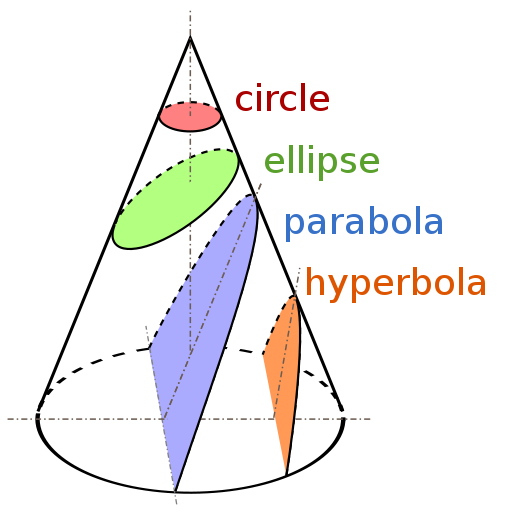
\includegraphics[width=5cm]{graphics/conic_sections.png}}\]
    \footnote{Figure taken from \url{https://en.wikipedia.org/wiki/File:Conic_Sections.svg}}
    % https://en.wikipedia.org/wiki/File:Conic_Sections.svg
\end{frame}

\begin{frame}{Affine Space}
    In Algebraic Geometry, our classical conic sections become part of affine spaces.
    \begin{block}{Definition}
    Let $k$ be a field, $n \geq 0$ an integer, the \textbf{affine space} of dimension $n$ is $k^n$, which we will denote as $\Abb^{n}_k$
    \end{block}
    
    \begin{block}{Definition}
    An (affine) \textbf{algebraic variety} $V \subset \Abb^{n}_k$ is the set of common $k$-roots of a collection of polynomials $\{F_i\}_{i \in I}$ where $F_i \in k[x_1, ..., x_n]$. We write $V$ as
    \[V = \Vbb(\{F_i\}_{i \in I})\]
    \end{block}
\end{frame}

\begin{frame}{Example of Affine Algebraic Varieties}
    
    \begin{block}{Example:}
        In the affine space $\Abb^{n}_k$
    \begin{itemize}
        \item $\Vbb(0) = \Abb^{n}_k$, $\Vbb(1) = \O$
        \item $\Vbb(x_1 - a_1, ..., x_n - a_n) = \{(a_1, ..., a_n)\}$
        \item Take $k = \Rbb, n = 2$, then the classical conic section $C$ is the variety
        \[C = \Vbb(ax^2 + by^2 + c + dxy + ey + fx)\]
        where $a, b, c, d, e, f \in \Rbb$
    \end{itemize}
    \end{block}
    
\end{frame}

\begin{frame}{Projective Space}
    The theory of affine varieties is great, but we can generalize conics with what's known as ``projective spaces".

    \begin{block}{Definition}
        The set of $1$-dimensional subspaces of $\Abb^{n+1}_k$ is called the \textbf{projective space} of dimension $n$, denoted as $\Pbb^n_k$. In other words, they are just the set of lines going through the origin in $\Abb^{n+1}_k$.
    \end{block}

    Notations:
     \begin{itemize}
         \item We will denote the line through $0$ and $(a_0, ..., a_{n})$ as $[a_0: ... : a_{n}]$ in $\Pbb^n_k$.
         \item Sometimes we will denote $\Pbb^n_k$ as $\Pbb^n_{k, [x_0, ..., x_{n}]}$ to emphasize its coordinates. 
     \end{itemize}

    % Equivalently, we can view the projective space as the quotient
    % \[\Pbb^n_k \cong \frac{\Abb^{n+1}_k - \{0\}}{\sim}\]
    % , where $(a_0, ..., a_{n}) \sim (b_0, ..., b_{n})$ if there exist some non-zero $\lambda \in k$ s.t.
    % \[\lambda(a_0, ..., a_{n}) = (b_0, ..., b_{n})\]
\end{frame}

\begin{frame}{Why Projective Spaces?}
    Q: Why do we want to study conics in projective spaces rather than affine spaces?\\
    \vspace{\baselineskip}
    A: There are 2 reasons:
    \begin{itemize}
        \item Geometrically, projective spaces are a natural compactification of affine spaces.
        \item Algebraically, we can turn conic sections into a class of what's called ``homogeneous polynomials", which is generally nicer to work with.
    \end{itemize}
\end{frame}

\begin{frame}{Embedding the Affine Plane}
     We can embed the affine plane $\Abb^2_k$ into $\Pbb^2_k$ by identifying $\Abb^2$ with the subset $U_Z = \{[X: Y: Z] \in \Pbb^2_k\ |\ Z \neq 0\}$ via:
     \[\varphi_Z: U_Z \to \Abb^2_k,\ [X: Y: Z] \mapsto (\frac{X}{Z}, \frac{Y}{Z}) \]
\[\frame{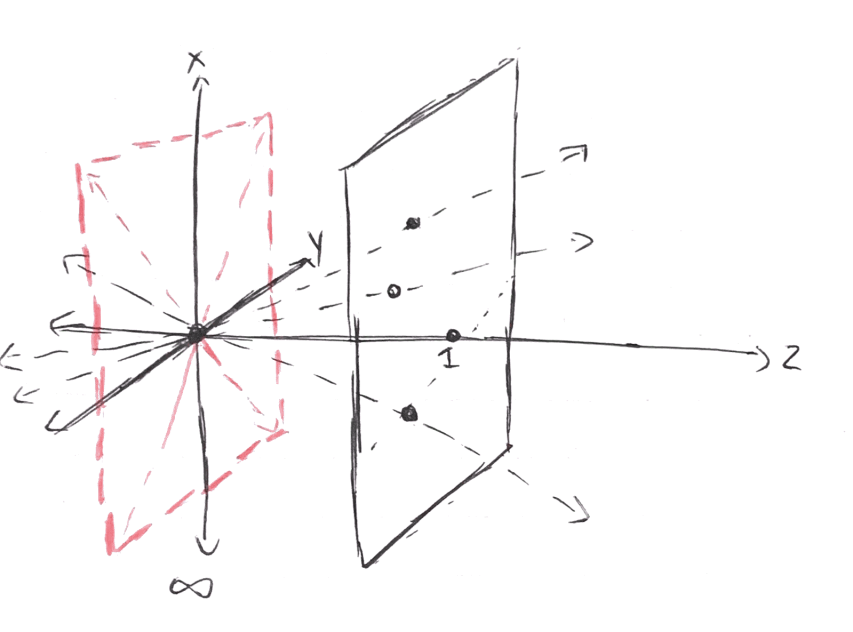
\includegraphics[width=6cm]{graphics/chart.png}}\]
This gives the compactification $\Pbb^2_k = \Abb^2_k \sqcup \Pbb^1_k$
\end{frame}

\begin{frame}{Homogeneous Polynomials}
    % Q: Why are we interested in projective spaces?\\
    % A: They serve as a convenient space to study the roots of a special class of polynomials.
    
    \begin{definition}
    A polynomial $F \in k[x_0, ..., x_n]$ is called \textbf{homogeneous of degree d} if it is a sum of degree $d$ monomials.
    \end{definition}
    For example, in $\Rbb[x, y, z]$, 
    \[6x^5 + 7y^5 + \pi x^4y + 3x^2y^2z + 9z^5\]
    is a homogeneous polynomial of degree $5$.
    
    \begin{block}{Observation:}
    Let $F$ be a homogeneous polynomial of degree $d$ and $\lambda \in k$,
    \[F(\lambda a_0, ..., \lambda a_n) =  \lambda^d F(a_0, ..., a_n)\]
    for all $(a_0, ..., a_n) \in k^{n+1}$. In particular, if $(a_0, ..., a_n)$ is a root of $F$, then so is $(\lambda a_0, ..., \lambda a_n)$.
    \end{block}
\end{frame}

\begin{frame}{Connection to Conics}
    Classically, conic sections have been considered as real roots of the polynomial
    \[f(x,y) = ax^2 + by^2 + c + dxy + ey + fx \in \Rbb[x, y]\]
    With our embedding, we can homogenize $f(x, y)$ into:
    \[F(X, Y, Z) = aX^2 + bY^2 + cZ^2 + dXY + eYZ + fXZ\]
    Then we note that on $Z = 1$, $F(X, Y, Z)$ becomes $f(x, y)$. This is in fact a bijective correspondence.
    
    \begin{block}{Definition:}
    Let $k$ be a field of characteristic $\neq 2$, a \textbf{plane conic} $C \subset \Pbb^2_{[X:Y:Z], k}$ is the $k$-roots of a homogeneous polynomial of degree 2 in $k[X, Y, Z]$.
    \end{block}
\end{frame}


\begin{frame}{Matrices and Conics}
Take any homogenous polynomial of degree $2$
\[F(X, Y, Z) := aX^2 + bY^2 + cZ^2 + dXY + eYZ + fXZ\]
We note that this polynomial has an associated symmetric matrix
\[M_F = \begin{bmatrix}
a & \frac{d}{2} & \frac{f}{2}\\
\frac{d}{2} & b & \frac{e}{2}\\
\frac{f}{2} & \frac{e}{2} & c
\end{bmatrix}\]
such that
\[F(X, Y, Z) = \begin{bmatrix} 
X & Y & Z
\end{bmatrix}
M_F
\begin{bmatrix} 
X\\
Y\\
Z
\end{bmatrix}\]
This also makes $F(X, Y, Z)$ into what's called a \textbf{quadratic form} of 3 variables.
\end{frame}

\begin{frame}{Smoothness of Conics}
It turns out that the rank of the matrix $M_F$ determines the geometry of the conic $C$. 
    \begin{block}{Fact: }
    Let $\overline{k}$ be the algebraic closure of $k$,
    \begin{itemize}
        \item If $M_F$ has rank $3$, then $C$ is a smooth conic
        \item If $M_F$ has rank $2$, then $C_{\overline{k}}$, by considering all $\overline{k}$-roots of $F$, is the union of two distinct lines meeting at a point.
        \item If $M_F$ has rank $1$, then $C_{\overline{k}}$ is a double line.
    \end{itemize}
    \end{block}
\end{frame}

\begin{frame}{Example: $rank(M_F) = 3$}

Let $k = \Rbb$, $M_F = \begin{bmatrix}
1 & 0 & 0\\
0 & 1 & 0\\
0 & 0 & -1
\end{bmatrix}$, $F(X, Y, Z) = X^2 + Y^2 - Z^2$.\\
Then $C$ is a smooth conic.\\
On the chart $(Z \neq 0)$,
     \[\frame{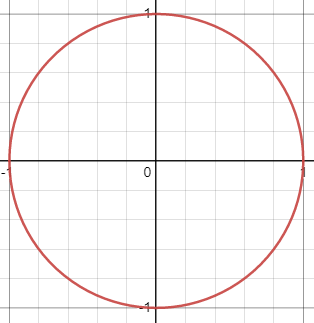
\includegraphics[width=5cm]{graphics/rank3.png}}\]
\end{frame}

\begin{frame}{Example: $rank(M_F) = 2$}
Let $k = \Rbb$, $M_F = \begin{bmatrix}
1 & 0 & 0\\
0 & -1 & 0\\
0 & 0 & 0
\end{bmatrix}$, $F(X, Y, Z) = X^2 - Y^2$.\\
Then $C$ is the union of two lines meeting at the origin.\\
On the chart $(Z \neq 0)$,
     \[\frame{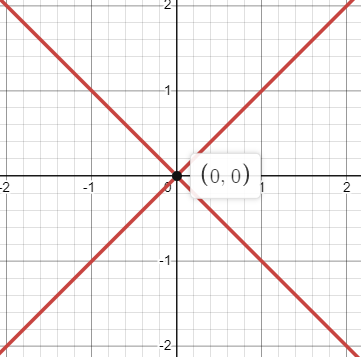
\includegraphics[width=5cm]{graphics/rank2.png}}\]
\end{frame}

\begin{frame}{Example: $rank(M_F) = 1$}
Let $k = \Rbb$, $M_F = \begin{bmatrix}
1 & 0 & 0\\
0 & 0 & 0\\
0 & 0 & 0
\end{bmatrix}$, $F(X, Y, Z) = X^2$.\\
Then $C$ is a line, we say it's ``double" because of the square.\\
On the chart $(Z \neq 0)$,
     \[\frame{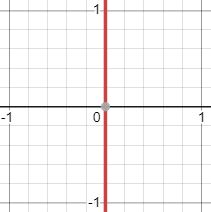
\includegraphics[width=5cm]{graphics/rank1.png}}\]
\end{frame}

\begin{frame}{Conic Bundles}

\begin{block}{Definition\footnote{We need a few more ideas in algebraic geometry to properly define conic bundles, but for the purpose of this talk we will adopt this more convenient definition.}:}
A \textbf{conic bundle} is a morphism $\pi: X \to S$ between (smooth) varieties $X, S$ such that the fiber of every point $p \in S$, defined as $\pi^{-1}(\{p\})$, is a conic, and the generic fiber is a smooth conic.
\end{block}



\end{frame}

\begin{frame}{Conic Bundles}
    \begin{block}{Example: }
    In our research, we are interested in the conic bundle $\pi: \Ydd \to \Pbb^2_{\Rbb, [u: v: w]}$ where:
    \begin{itemize}
        \item $\Ydd$ is a variety defined by the equation:
    \[z^2 = Q_1(u, v, w) t_0^2 + 2Q_2(u, v, w) t_0t_1 + Q_3(u, v, w) t_1^2\]
        \item $Q_1, Q_2, Q_3 \in \Rbb[u, v, w]$ are homogenous polynomials of degree $2$
        \item $\pi$ is the standard projection
    \end{itemize}
        \[\begin{tikzcd}[ampersand replacement=\&]
	{\Ydd} \\
	{{\mathbb{P}^1_{\Rbb, [t_0:t_1]} \times \mathbb{P}^2_{\Rbb, [u:v:w]} }} \& {\mathbb{P}^2_{\Rbb, [u:v:w]}}
	\arrow[from=1-1, to=2-1]
	\arrow[from=2-1, to=2-2]
	\arrow["{\pi}", from=1-1, to=2-2]
\end{tikzcd}\]
    \end{block}

\end{frame}

\begin{frame}{Why is $\pi$ a conic bundle?}
Intuitively, for a conic bundle $\pi: X \to S$, every point in $S$ should correspond to some conic in $X$. 
   \begin{block}{Example of Fibers for $\pi$:}
   Concretely, take the point ${\color{red}[1 : 2 : 3]} \in \Pbb^2_{\Rbb,[u:v:w]}$, then fiber of ${\color{red}[1 : 2 : 3]}$ is exactly the solutions satisfying:
   \[z^2 = Q_1({\color{red}1, 2, 3})t_0^2 + 2Q_2({\color{red}1, 2, 3})t_0t_1 + Q_3({\color{red}1, 2, 3})t_1^2\]
   This forms a conic in $\Pbb^2_{\Rbb, [t_0:t_1:z]}$.
   \end{block}
    Thus, $\pi: \Ydd \to \Pbb^2_{\Rbb, [u: v: w]}$ is an example of a \textbf{conic bundle}. 
%     \begin{block}{Question:}
% What if we try to project down to $[t_0: t_1]$ instead?
% \end{block}
\end{frame}

% \begin{frame}{The Quadric Surface Bundle}
% Let $\pi_1: \Ydd \to \Pbb^1_{[t_0, t_1]}(\Rbb)$ be the projection map described
%   \begin{block}{Example of Fibers for $\pi_1$:}
%   Similarly, take the point ${\color{red} [1:3]} \in \Pbb^1_{[t_0: t_1]}(\Rbb)$, then fiber of ${\color{red} [1:3]}$ is exactly the solutions satisfying:
%   \[z^2 = Q_1(u, v, w){\color{red}(1)^2} + 2Q_2(u, v, w){\color{red}(1)(3)} + Q_3(u, v, w){\color{red}(3)^2}\]
%   \[= {\color{red}(1)}Q_1(u, v, w) + 2{\color{red}(3)}Q_2(u, v, w) + {\color{red}(9)}Q_3(u, v, w)\]
%   This forms a degree 2 surface (known as a \textbf{quadric}) in $\Pbb^3_{[u:v:w:z]}(\Rbb)$.
%   \end{block}
%     Thus, $\pi_1: \Ydd \to \Pbb^1_{[t_0: t_1]}(\Rbb)$ is an example of a \textbf{quadric surface bundle}. 
% \end{frame}

% \begin{frame}{Conic Bundles (Continued)}
%     Putting $\pi_1$ and $\pi_2$ together, we have the commutative diagram:
%         \[\begin{tikzcd}[ampersand replacement=\&]
% 	\& {Y_{\tilde{\Delta}/\Delta}} \\
% 	\& {\mathbb{P}^1_{[t_0:t_1]}(\mathbb{R}) \times \mathbb{P}^2_{[u:v:w]}(\mathbb{R})} \\
% 	{\mathbb{P}^1_{[t_0:t_1]}(\mathbb{R})} \&\& {\mathbb{P}^2_{[u:v:w]}(\mathbb{R})}
% 	\arrow[from=1-2, to=2-2]
% 	\arrow[from=2-2, to=3-1]
% 	\arrow["{\pi_1}"', curve={height=12pt}, from=1-2, to=3-1]
% 	\arrow[from=2-2, to=3-3]
% 	\arrow["{\pi_2}", curve={height=-12pt}, from=1-2, to=3-3]
% \end{tikzcd}\]
% \end{frame}

\begin{frame}{The Discriminant Curve}
We would like to identify if a given fiber of $\pi$ is smooth:
    \begin{block}{Smoothness Criterion}
       Given fixed $[u: v: w] \in \Pbb^2_{\Rbb, [u: v: w]}$, we can rewrite its assoicated conic as:
       \[0 = {\color{red}Q_1(u, v, w)}t_0^2 + {\color{red}2Q_2(u, v, w)}t_0t_1 + {\color{red}Q_3(u, v, w)}t_1^2 + {\color{red}(-1)}z^2\ (*)\]
       This gives the symmetric matrix:
       \[M = \begin{bmatrix}
       Q_1(u, v, w) & Q_2(u, v, w) & 0\\
       Q_2(u, v, w) & Q_3(u, v, w) & 0\\
       0 & 0 & -1
       \end{bmatrix}\]
       The conic $(*)$ is smooth if and only if $\det(M) \neq 0$.
    \end{block}
\end{frame}

\begin{frame}{The Discriminant Curve}
    \begin{block}{Smoothness Criterion (Continued):}
    The curve defined by $\det(M) = 0$ is called the \textbf{discriminant curve} $\Delta$:
    \[\Delta = (Q_1Q_3 - Q_2^2 = 0) \subset \Pbb^2_{[u: v: w]}\]
    \end{block}

\begin{figure}[h]
    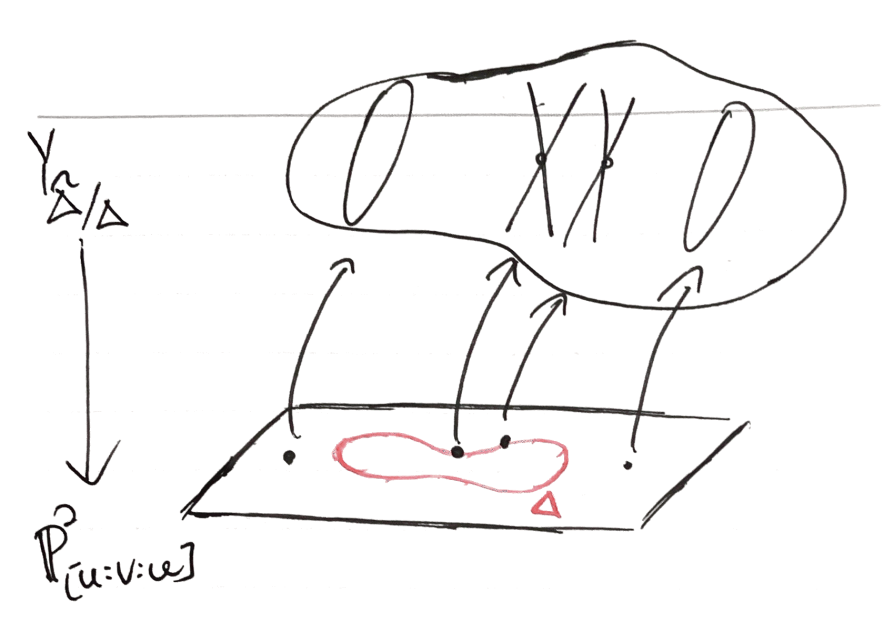
\includegraphics[width=7cm]{graphics/conic_bundle.png}
\end{figure}
\end{frame}


\begin{frame}{Quartic Plane Curves}
$Q_1Q_3 - Q_2^2$ is a degree 4 homogeneous real polynomial.
\begin{definition}
The roots of a degree 4 homogenous polynomial over $\Pbb^2_\Rbb$ is known as a \textbf{quartic}.
\end{definition}
        \begin{block}{Theorem (Zeuthen, 1874)}
       Let $\Delta$ be a smooth quartic over $\Rbb$, then $\Delta(\Rbb)$ can be classified into 1 of the 6 following topological types:
       \begin{enumerate}
           \item No real points
           \item One oval
           \item Two nested ovals
           \item Two non-nested ovals
           \item Three ovals
           \item Four ovals
       \end{enumerate}
        \end{block}
\end{frame}

\begin{frame}{Example: Four Ovals}

 The homogeneous equation defines a smooth quartic whose real component has 4 ovals:
 \[0 = \frac{509}{18}x^4 - \frac{6397}{114}x^2y^2 + \frac{2219}{76}y^4 - \frac{2203}{102}x^2z^2 + \frac{4011}{323}y^2z^2 + \frac{2123}{289}z^4\]
The real components on the chart $(z \neq 0)$
 \[\frame{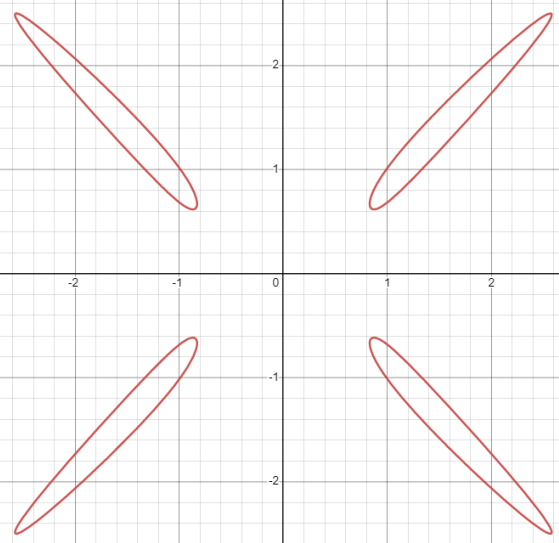
\includegraphics[width=5cm]{graphics/4ovals.png}}\]
    
\end{frame}

\begin{frame}{Example: Two Nested Ovals}
This homogeneous equation defines a smooth quartic whose real component has 2 nested ovals:
 \[0 = -3x^4 - \frac{7}{10}x^2y^2 - \frac{169}{400}y^4 + \frac{67}{6}x^2z^2 + \frac{949}{240}y^2z^2 - \frac{121}{576}z^4\]
The real components on the chart $(z \neq 0)$:
 \[\frame{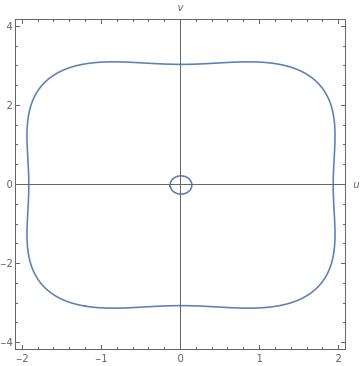
\includegraphics[width=5cm, height=5cm]{graphics/nested.png}}\]
\end{frame}

\begin{frame}{Connectedness}
\begin{block}{Remark:}
    Our work at this REU so far has been investigating the relationship between the topological type of $\Delta(\Rbb)$ and various properties of $\Ydd(\Rbb)$
\end{block}

One interesting property we have been investigating so far is the question of connectedness.

% \begin{definition}
% We say $\Ydd$ is \textbf{$\Rbb$-rational} if there are open subsets $U \subset \Ydd$ and $V \subset \Pbb^3(\Rbb)$ such that $U$ and $V$ are isomorphic.
% \end{definition}

% \begin{block}{Fact:}
% If $\Ydd$ is $\Rbb$-rational, then $\Ydd(\Rbb)$ is connected.
% \end{block}

\end{frame}

\begin{frame}{Some Results So Far}
    
    \begin{theorem}
    With the previous setup of $\Ydd(\Rbb)$
    \begin{itemize}
        \item $\Ydd(\Rbb)$ has at most $3$ connected components
        \item If the topological type of $\Delta(\Rbb)$ is empty, $1$ oval, or $4$ ovals, then $\Ydd(\Rbb)$ is connected
        \item If $\Ydd(\Rbb)$ has $2$ connected components, then $\Delta(\Rbb)$ is either $2$ nested ovals or $2$ non-nested ovals
        \item If $\Ydd(\Rbb)$ has $3$ connected components, then $\Delta(\Rbb)$ is $3$ ovals
    \end{itemize}
    \end{theorem}
    
    \begin{proof}
     Exercise :)
    \end{proof}

\end{frame}

% \begin{frame}{Acknowledgements}
%     \begin{itemize}
%         \item [1] Atiyah, Michael Francis and MacDonald, I. G.. ``Introduction to commutative algebra" Addison-Wesley-Longman, 1969.
%         \item [2] Bradley, Tai-Danae. ``The Yoneda Lemma.” RSS, https://www.math3ma.com/blog/the-yoneda-lemma.
%         \item [3] Riehl, Emily. ``Category Theory in Context" Dover, 2016.
%     \end{itemize}
% \end{frame}
\end{document}